\documentclass[submit]{../harvardml}

\course{CS1810-S25}
\assignment{Homework \#2}
\duedate{February 28, 2025 at 11:59 PM}

\usepackage{../common}
\usepackage[OT1]{fontenc}
\usepackage[colorlinks,citecolor=blue,urlcolor=blue]{hyperref}
\usepackage{graphicx}
\usepackage{subfig}
\usepackage{fullpage}
\usepackage{amsmath}
\usepackage{amssymb}
\usepackage{framed}
\usepackage{color}
\usepackage{soul}
\usepackage{todonotes}
\usepackage{listings}
\usepackage{enumitem}
\usepackage{bm}
\usepackage{bbm}
\usepackage{float}


\newcommand{\B}{\text{B}}
\newcommand{\Beta}{\text{Beta}}

\usepackage[mmddyyyy,hhmmss]{datetime}

\definecolor{verbgray}{gray}{0.9}

\lstnewenvironment{csv}{%
  \lstset{backgroundcolor=\color{verbgray},
  frame=single,
  framerule=0pt,
  basicstyle=\ttfamily,
  columns=fullflexible}}{}
  

%%%%%%%%%%%%%%%%%%%%%%%%%%%%%%%%%%%%%%%%%%%
%% Solution environment
\usepackage{xcolor}
\newenvironment{solution}{
    \vspace{2mm}
    \color{blue}\noindent\textbf{Solution}:
}{}
%%%%%%%%%%%%%%%%%%%%%%%%%%%%%%%%%%%%%%%%%%%


\begin{document}

\begin{center}
  {\Large Classification and Bias-Variance Trade-offs}\\
\end{center}

\subsection*{Introduction}

This homework is about classification, bias-variance trade-offs, and
uncertainty quantification.

The datasets that we will be working with relate to astronomical observations and loan applicants
The first dataset, found at \verb|data/planet-obs.csv|,
contains information on whether a planet was observed (as a binary
variable) at given points in time. This will be used in Problem 1. The
second dataset, available at \verb|data/hr.csv|, details different
loan applicants and their measured debt to income ratio and credit score. You will
work with this data in Problem 3.

As a general note, for classification problems we imagine that we have
the input matrix $\boldX \in \reals^{n \times d}$ (or perhaps they
have been mapped to some basis $\bm{\Phi}$, without loss of
generality) with outputs now ``one-hot encoded."  This means that if
there are~$K$ output classes, rather than representing the output
label $y$ as an integer~${1,2,\ldots,K}$, we represent $\boldy$ as a
``one-hot" vector of length~$K$. A ``one-hot" vector is defined as
having every component equal to 0 except for a single component which
has value equal to 1.  For example, if there are $K = 7$ classes and a
particular data point belongs to class 3, then the target vector for
this data point would be~$\boldy = [0,0,1,0,0,0,0]$.  We will define
$C_1$ to be the one-hot vector for the 1st class, $C_2$ for the 2nd
class, etc.  Thus, in the previous example $\boldy = C_3$. If there
are $K$ total classes, then the set of possible labels is $\{C_1
  \ldots C_K \} = \{C_k\}_{k=1}^K$.  Throughout the assignment we will
assume that each label $\boldy \in \{C_k\}_{k=1}^K$ unless otherwise
specified. The most common exception is the case of binary
classification ($K = 2$), in which case labels are the typical
integers $y \in \{0, 1\}$.

\subsection*{Resources and Submission Instructions}

We encourage you to read CS181 Textbook's Chapter 3 for more
information on linear classification, gradient descent, and
classification in the discriminative setting. Read Chapter 2.8 for
more information on the trade-offs between bias and variance.

In problems 1 and 3, you may use \texttt{numpy} or \texttt{scipy}, but
not \texttt{scipy.optimize} or \texttt{sklearn}. Example code is given
in the provided notebook. \textbf{We highly recommend that you use Google Colab for problems 1 and 3 to avoid numerical stability issues.}

Please type your solutions after the corresponding problems using this
\LaTeX\ template, and start each problem on a new page.

Please submit the \textbf{writeup PDF to the Gradescope assignment
  `HW2'}. Remember to assign pages for each question.  Please submit
your \textbf{\LaTeX\ file and code files to the Gradescope assignment
  `HW2 - Supplemental'}. \textbf{You must include your plots in your
  writeup PDF. } The supplemental files will only be checked in
special cases, e.g. honor code issues, etc.


%%%%%%%%%%%%%%%%%%%%%%%%%%%%%%%%%%%%%%%%%%%%%
% Problem 1
%%%%%%%%%%%%%%%%%%%%%%%%%%%%%%%%%%%%%%%%%%%%%

\begin{problem}[Exploring Bias-Variance and Uncertainty]
In this problem, we will explore the bias and variance of a few
different model classes when it comes to logistic regression and
investigate two sources of predictive uncertainty in a synthetic
(made-up) scenario.

We are using a powerful telescope in the northern hemisphere to gather
measurements of some planet of interest. At certain times however, our
telescope is unable to detect the planet due to its positioning around
its star.  The data in \verb|data/planet-obs.csv| records the
observation time in the ``Time" column and whether the planet was
detected in the ``Observed" column (with the value 1 representing that
it was observed).  These observations were taken over a dark, clear
week, which is representative of the region.  Since telescope time is
expensive, we would like to build a model to help us schedule and find
times when we are likely to detect the planet.

\begin{enumerate}
  \item Split the data into 10 mini-datasets of size $N = 30$ (i.e. dataset 1 consists of the first 30 observations, dataset 2 consists of the next 30, etc. This has already been done for you). Consider the three bases $\boldsymbol\phi_1(t) = [1, t]$, $\boldsymbol\phi_2(t) = [1,
          t, t^2]$, and $\boldsymbol\phi_3(t) = [1, t, t^2, t^3, t^4, t^5]$. For each of these bases, fit a logistic regression model using sigmoid($\boldw^\top \boldsymbol\phi(t)$) to each dataset by using gradient descent to
        minimize the negative log-likelihood.  This means you will be
        running gradient descent 10 times for each basis, once for each
        dataset.

        Use the given starting values of $\boldw$ and a learning rate of $\eta=0.001$, take 1,000 update
        steps for each gradient descent run, and make sure to average the
        gradient over the data points at each step. These parameters,
        while not perfect, will ensure your code runs reasonably quickly.

  \item After consulting with a domain expert, we find that the probability of observing the planet is periodic as the planet revolves around its star---we are more likely to observe the planet when it is in front of its star than when it is behind it. In fact, the expert determines that observation follows the generating process $y \sim \text{Bern}(f(t))$, where $f(t) = 0.4 \times \cos(1.1t + 1) + 0.5$ for $t \in [0, 6]$ and $y \in \{0,1\}$. Note that we, the modelers, do not usually see the true data distribution. Knowledge of the true $f(t)$ is only exposed in this problem to allow for verification of the true bias.

        Use the given code to plot the true process versus your learned models. Include your plots in your solution PDF.

        \textbf{In no more than 5 sentences}, explain how bias and variance reflected in the 3 types of curves on the graphs.  How do the fits of the individual and mean prediction functions change?  Keeping in mind that none of the model classes match the true generating process exactly, discuss the extent to which each of the bases approximates the true process.

\end{enumerate}
\end{problem}

\newpage
\begin{framed}
  \noindent\textbf{Problem 1} (cont.)\\
  \begin{enumerate}
    \setcounter{enumi}{2}

    \item If we were to increase the size of each dataset drawn from $N = 30$ to a larger number, how would the bias and variance change for each basis? Why might this be the case? You may experiment with generating your own data that follows the true process and plotting the results, but this is \textbf{not} necessary. \textbf{Your response should not be longer than 5 sentences}.

    \item Consider the test point $t = 0.1$. Using your models trained on basis $\boldsymbol\phi_3$, report the predicted probability of observation of the \textit{first} model (the model trained on the first 30 data points). How can we interpret this probability as a measure of uncertainty? Then, compute the variance of the classification probability over your 10 models at the same point $t = 0.1$. How does this measurement capture another source of uncertainty, and how does this differ from the uncertainty represented by the classification probability? Repeat this process (reporting the first model's classification probability and the variance over the 10 models) for the point $t = 3.2$.

          Compare the uncertainties and their sources at times $t=0.1$ and $t=3.2$.

    \item We now need to make some decisions about when to request time on
          the telescope.  The justifications of your decisions will be sent to
          your funding agency, which will determine whether you will be
          allocated funds to use the telescope for your project. \textbf{In no more than 10 lines}, answer the following questions.
          \begin{itemize}
            \item To identify the ideal time, which model(s) would you use and why?
            \item What time would you request, and why?
            \item Your funding agency suggests using a different telescope in a
                  humid area near the equator. Can you still use your model to
                  determine when the planet is likely to be visible?  Why? Are there
                  adaptations that may be necessary?
            \item You seek out a team that has used the alternative telescope
                  for observing this planet, and they provide you their observation
                  file \verb|data/planet-obs-alternate.csv|.
                  Compare the observations from your telescope to theirs.  What
                  seems to be happening?  What might be an appropriate model for
                  this? Your funding agency asks you to refit your models on these
                  new data.  Do you think this is a reasonable ask, and if so, how
                  will it help you make better decisions about when to request
                  viewing time?  If not, why do you think the additional modeling
                  will not help? You do \emph{not} need to do any modeling for this
                  question!

          \end{itemize}
          In these questions, we are looking for your reasoning; there may be
          more than one valid answer.

  \end{enumerate}
\end{framed}

\newpage

\begin{solution}

\begin{enumerate}
    \item From 3.14 in the textbook, we can find our gradient of cross-entropy loss as:

    \[
    \nabla L(w) = \sum_{i=1}^N(\hat y_i - y_i)x_i
    \]

    where $\hat y_i = \sigma(w^\top x_i)$. Thus we can write this as

    \[
    \nabla L(w) = X^\top (\hat y - y)
    \]

    Therefore we can perform gradient descent as

    \[
    w_{new} \leftarrow w_{old} - \eta \nabla L(w)
    \]

    and our prediction is $\hat y=\sigma(Xw)$ where the function acts on each component of the vector.

    \item We can see from the plots that our graphs with more features tend to have less bias and more variance. The basis 1 graph has the most bias and least variance, the basis 2 graph has a moderate amount of bias and more variance, and the basis 3 graph has less bias and the most variance (as seen above). The fits seem to become more accurate and mean prediction functions seem to more closely match the ground truth, with the bases seeming to approximate the true process better as the number of features increases.

    \begin{figure}[H]
        \centering
        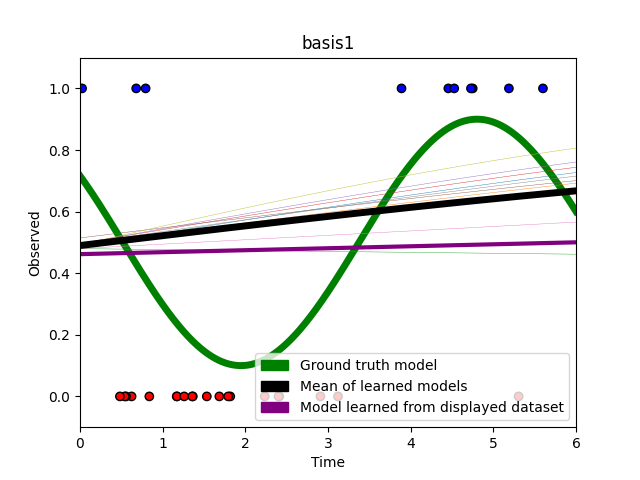
\includegraphics[width=0.5\linewidth]{basis1.png}
    \end{figure}

    \begin{figure}[H]
        \centering
        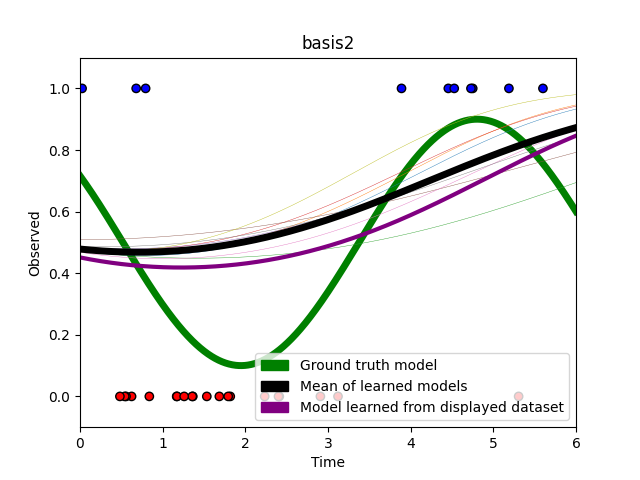
\includegraphics[width=0.5\linewidth]{basis2.png}
    \end{figure}

    \begin{figure}[H]
        \centering
        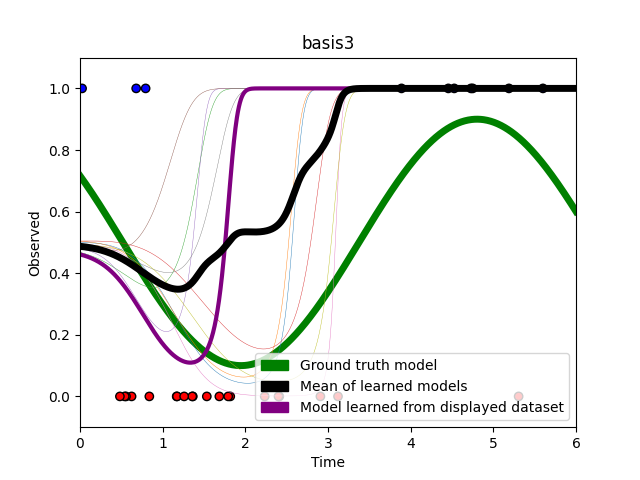
\includegraphics[width=0.5\linewidth]{basis3.png}
    \end{figure}


    \item For the first bases, increasing the size of the dataset would likely result in it maintaining a high bias and low variance since it results in a linear model, which cannot really capture the periodic behavior of the ground truth. For the second basis, the extra data may allow for the models to decrease bias and increase variance, better fitting to the data due to the increased flexibility from it being a quadratic model. Finally for the last basis, the bias would likely decrease and variance decrease as well since the model has more data to fit properly. With small amounts of data, the higher order polynomial model would likely overfit, so by increasing the data, we can reduce overfitting by decreasing variance, which would result in a better model. 

    \item At $t = 0.1$, our first model reports a classification probability of $0.4989$, which indicates a decent amount of uncertainty since the probability was nearly 0.5. In contrast, our first model's classification probability of $t=3.2$ was $0.9999$, which indicates low uncertainty since the probability is nearly 1. Across the 10 models, we can find the variance for both time points. At $t=0.1$, the variance was $0.000278$ which suggests that the models are consistently uncertain in the classification for that time point. Similarly, at $t=3.2$, the variance was $0.205$ which is much larger than that of $t=0.1$, indicating that the model is fairly inconsistent in the classification. Compared to the models' results for $t=0.1$, the models' predictions for $t=3.2$ are less in agreement but more confident in their individual classifications.

    \item We will use model 3 to identify the ideal time as it best approximates the periodic nature of the data and have enough features that we will not be missing crucial datapoints, staying cautious of overfitting. From the model, we would request times from 3-6 since that is when the mean of learned models indicates that we will observe the planet (which is fairly accurate to the truth. We cannot use our model to determine when the planet is likely to be visible in a humid area near the equator since there would likely be more cloud coverage, reducing visiblity. We would need to retrain the model on local data if we were to move it to a different location to account for potential weather complexities. The data from the alternate telescope is plotted below. We can see that the data is sporadic and doesn't follow the same periodic pattern as the previous data, so fitting a model to the alternative telescope data does not help and would rather be more harmful. Thus the ask is unreasonable.

    

    \begin{figure}[H]
        \centering
        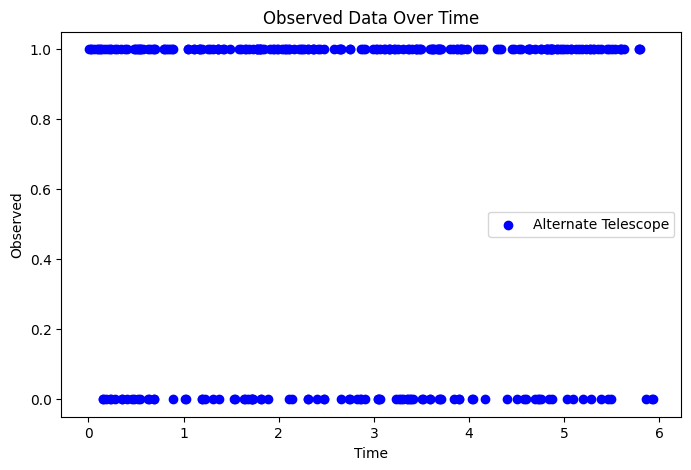
\includegraphics[width=0.5\linewidth]{alternate.png}
    \end{figure}

    \begin{figure}[H]
        \centering
        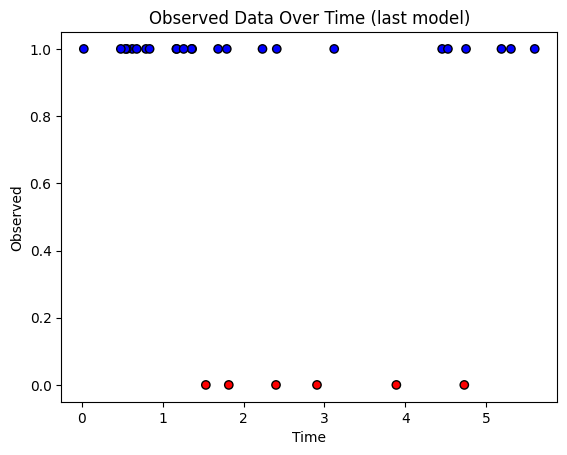
\includegraphics[width=0.5\linewidth]{pelase.png}
    \end{figure}
    
\end{enumerate}

\end{solution}

%%%%%%%%%%%%%%%%%%%%%%%%%%%%%%%%%%%%%%%%%%%%%
% Problem 2
%%%%%%%%%%%%%%%%%%%%%%%%%%%%%%%%%%%%%%%%%%%%%

\begin{problem}[Maximum likelihood in classification]

Consider now a generative $K$-class model.  We adopt class prior
$p(\boldy = C_k; \bpi) = \pi_k$ for all $k \in \{1, \ldots, K\}$
(where $\pi_k$ is a parameter of the prior).
Let  $p(\boldx|\boldy=C_k)$ denote
the class-conditional density of features $\boldx$ (in this
case for class $C_k$). Consider the data set $D = \{(\boldx_i,
  \boldy_i)\}_{i=1}^n$ where as above $\boldy_i \in \{C_k\}_{k=1}^K$ is
encoded as a one-hot target vector and the data are independent.

\begin{enumerate}
  \item Write out the log-likelihood of the data set, $\ln p(D ; \bpi)$.

  \item Since the prior forms a distribution, it has the constraint that
        $\sum_k\pi_k - 1 = 0$.  Using the hint on
        Lagrange multipliers below, give the
        expression for the maximum-likelihood estimator for the prior
        class-membership probabilities, i.e.
        $\hat \pi_k.$
        Make sure to write out the intermediary equation you need
        to solve to obtain this estimator. Briefly state why your final answer is intuitive.
\end{enumerate}

For the remaining questions, let the
class-conditional probabilities be Gaussian distributions with
the same covariance matrix
$$p(\boldx | \boldy = C_k) = \mathcal{N}(\boldx |  \bmu_k, \bSigma), \text{\ for\ }k \in \{1,\ldots, K\}$$
and different means $\bmu_k$ for each class.

\begin{enumerate}
  \item[3.] Derive the gradient of the log-likelihood with respect to vector $\bmu_k$.
    Write the expression in matrix form as a function of the variables defined
    throughout this exercise. Simplify as much as possible for full credit.
  \item[4.] Derive the maximum-likelihood estimator $\hat{\mu}_k$ for vector $\bmu_k$. Briefly state why your final answer is intuitive.
  \item[5.] Derive the gradient for the log-likelihood with respect to the
    covariance matrix $\bSigma$ (i.e., looking
    to find an MLE for the covariance).
    Since you are differentiating with respect to a
    \emph{matrix}, the resulting expression should be a matrix!
    %
  \item[6.] Derive the maximum likelihood estimator $\hat{\Sigma}$ of the covariance matrix.
\end{enumerate}

\paragraph{Hint: Lagrange Multipliers.} Lagrange Multipliers are a method for
optimizing a function $f$ with respect to an
equality constraint, i.e.
\[\min_{\boldx} f(\boldx)\ \text{s.t.}\ g(\boldx) = 0.\]

This can be turned into an unconstrained problem by introducing a
Lagrange multiplier $\lambda$ and constructing the Lagrangian function,
\[L(\boldx, \lambda) =  f(\boldx) + \lambda g(\boldx).\]

It can be shown that it is a necessary condition that the optimum
is a critical point of this new function. We can find this point by solving two equations:

\[\frac{\partial L(\boldx, \lambda)}{\partial  \boldx} = 0  \ \ \text{and}\  \  \frac{\partial L(\boldx, \lambda)}{\partial \lambda} = 0 \]


\paragraph{Cookbook formulas.} Here are some formulas you might want to consider
using to compute difficult gradients. You can use them  in the homework
without proof. If you are looking to hone your matrix calculus skills, try to
find different ways to prove these formulas yourself (will not be part of the
evaluation of this homework). In general, you can use any formula from the matrix cookbook,
as long as you cite it. We opt for the following common notation:
$\boldX^{-\top} := (\boldX^{\top})^{-1}$
\begin{align*}
   & \frac{\partial \bolda^\top \boldX^{-1} \boldb}{\partial \boldX} = - \boldX^{-\top} \bolda \boldb^\top \boldX^{-\top} \\
   & \frac{\partial \ln | \det (\boldX) |}{\partial \boldX} = \boldX^{-\top}
\end{align*}
\end{problem}

\newpage

\begin{solution}

\begin{enumerate}
    \item We want to find $\ln p(D ; \bpi)$. Let $I(\cdot)$ represent the indicator for the event inside the parentheses. We can see that
    \begin{align*}
        p(D ; \bpi) &= \prod_{i=1}^n p(x_i, y_i ; \bpi) \\
        &= \prod_{i=1}^n \prod_{k=1}^K (p(x_i, y_i = C_k; \bpi))^{I(y_i = C_k)} \\
        &= \prod_{i=1}^n \prod_{k=1}^K (p(x | y_i = C_k)\pi_k)^{I(y_i=C_k)}
    \end{align*}

    since for $y$ is one-hot encoded so in each $y_i$ will belong to only one class. If it is not in the class, the indicator variable will result in the expression being $1$. Taking the log,

    \begin{align*}
        \ln p(D ; \bpi) &= \sum_{i=1}^n \ln\left(\left(\prod_{k=1}^Kp(x | y_i = C_k)\pi_k\right)^{I(y_i=C_k)}\right) \\
        &= \sum_{i=1}^n\sum_{k=1}^K I(y_i=C_k)\left(\ln(p(x|y_i=C_k)+\ln \pi_k\right) \\
        &=\boxed{\sum_{i=1}^n\sum_{k=1}^K I(y_i=C_k)\ln(p(x|y_i=C_k) + \sum_{i=1}^n\sum_{k=1}^K I(y_i=C_k) \ln \pi_k}
    \end{align*}

    \item We can use the Lagrange Multipliers to optimize $f$ with respect to each of the $\pi_k$. Since $\sum_{i=1}^n\sum_{k=1}^K I(y_i=C_k)\ln(p(x|y_i=C_k)$ doesn't contain $\pi_k$, we can write our Lagrangian function as

    \[
    L(\bpi, \lambda) = \sum_{i=1}^n \sum_{k=1}^K I(y_i = C_k) \ln \pi_k + \lambda \left(\sum_{k=1}^K \pi_k - 1\right)
    \]

    according to our constraint above. Therefore, we can find a critical point by setting the partials to 0. Since the derivative with respect to $\bpi$ is a vector of elements which are the partials with respect to some $\pi_j$, we can find each one:

    \[
    \frac{\partial L(\bpi, \lambda)}{\partial \pi_j} = \sum_{i=1}^n \frac{I(y=C_j)}{\pi_j} + \lambda = 0
    \]

    since the partial with respect to $\pi_j$ is nonzero only when $j=k$. We can solve for $\pi_j$

    \[
    \sum_{i=1}^n \frac{I(y=C_j)}{\pi_j} = - \lambda
    \]
    \[
    \pi_j = -\frac{1}{\lambda} \sum_{i=1}^n I(y_i = C_j)
    \]

    Solving for the partial with respect to $\lambda$,

    \begin{align*}
        \frac{\partial L(\bpi, \lambda)}{\partial \lambda} = \sum_{k=1}^K \pi_k - 1 &= 0 \\
        \sum_{k=1}^K \pi_k &= 1 \\
        \sum_{k=1}^K \left(-\frac{1}{\lambda} \sum_{i=1}^n I(y_i = C_k)\right) &= 1 \\
        -\frac{1}{\lambda}\sum_{k=1}^K \sum_{i=1}^n I(y_i = C_k) &= 1 \\
        -\frac{n}{\lambda} &= 1 \\
        \lambda &= -n
    \end{align*}

    since each of the indicators will be equal to 1 exactly once for a specific class. Substituting this into our expression for $\pi_j$:

    \[
    \pi_j = \frac{-1}{-n}\sum_{i=1}^n I(y_i = C_j)
    \]

    Let $n_j$ represent the number of samples in class $j$, then we can rewrite $\pi_j$ as

    \[
    \boxed{\hat \pi_j = \frac{\sum_{i=1}^nI(y_i = C_j)}{n}= \frac{n_j}{n}}
    \]

    Our final answer for our priors for each class makes sense since we would expect the prior probability for any class $j$ to be the proportion of the data that is from class $j$. This is what we observe above where our priors are just relative probabilities, which we use as an estimate.

    \item Recall that our expression for the log-likelihood was:

    \[
    \sum_{i=1}^n\sum_{k=1}^K I(y_i=C_k)\ln(p(x|y_i=C_k) + \sum_{i=1}^n\sum_{k=1}^K I(y_i=C_k) \ln \pi_k
    \]

    Given that our class-conditional probabilities are Gaussian distributions with the same covariance matrix, we can write:

    \[
    p(x_i | y_i = C_k) = \frac{1}{(2\pi)^{D/2}|\Sigma|^{1/2}}\exp\{-\frac{1}{2}(x_i - \mu_k)^\top \Sigma^{-1} (x_i - \mu_k)\}
    \]

    Therefore, we can write

    \begin{align*}
        \ln p(D;\bpi) &= \sum_{i=1}^n\sum_{k=1}^K I(y_i=C_k)\ln\left[\frac{1}{(2\pi)^{D/2}|\Sigma|^{1/2}}\exp\{-\frac{1}{2}(x_i - \mu_k)^\top \Sigma^{-1} (x_i - \mu_k)\}\right] + \sum_{i=1}^n\sum_{k=1}^K I(y_i=C_k) \ln \pi_k \\
        &= \sum_{i=1}^n\sum_{k=1}^K I(y_i=C_k)\left[ -\frac{D}{2} \ln (2\pi) - \frac{1}{2} \ln (|\Sigma|) -\frac{1}{2}(x_i - \mu_k)^\top \Sigma^{-1} (x_i - \mu_k)\right] + \sum_{i=1}^n\sum_{k=1}^K I(y_i=C_k) \ln \pi_k
    \end{align*}

    Taking the partial with respect to $\mu_k$:

    \begin{align*}
        \frac{\partial\ln p (D;\bpi)}{\partial \mu_k} &= \frac{\partial}{\partial \mu_k} \left(\sum_{i=1}^n\sum_{k=1}^K I(y_i=C_k)\left[-\frac{1}{2}(x_i - \mu_k)^\top \Sigma^{-1} (x_i - \mu_k)\right]\right) \\
        &= -\frac{1}{2} \sum_{i=1}^n I(y_i = C_k) \left[-2 \Sigma^{-1}(x_i - \mu_k)\right] \\
        &= \sum_{i=1}^n I(y_i = C_k) \Sigma^{-1}(x_i - \mu_k)
    \end{align*}

    which we know the identities from the Matrix Cookbook. Similar to above, let $n_k$ be the number of samples of class $k$. We know our sample mean can be found by:

    \[
    \bar{x}_k = \frac{1}{n_k} \sum_{i=1}^n I(y_i = C_k) x_i
    \]

    which we can substitute by definition below

    \begin{align*}
        \sum_{i=1}^n I(y_i = C_k) \Sigma^{-1}(x_i - \mu_k) &= \Sigma^{-1}\sum_{i=1}^n I(y_i = C_k) (x_i - \mu_k) \\
        &= \Sigma^{-1} \left(\sum_{i=1}^n I(y_i = C_k) x_i - \sum_{i=1}^n I(y_i = C_k) \mu_k\right) \\
        &= \Sigma^{-1}(n_k\bar{x}_k - n_k\mu_k) \\
        &= n_k \Sigma^{-1}(\bar{x}_k - \mu_k)
    \end{align*}

    Therefore,

    \[
    \boxed{\frac{\partial\ln p (D;\bpi)}{\partial \mu_k}  = n_k \Sigma^{-1}(\bar{x}_k - \mu_k)}
    \]

    \item To find the MLE $\bar{\mu}_k$, we can set the gradient to zero.

    \[
    \frac{\partial\ln p (D;\bpi)}{\partial \mu_k}  = 0
    \]
    \[
    n_k \Sigma^{-1}(\bar{x}_k - \mu_k) = 0
    \]
    \[
    n_k (\bar{x}_k - \mu_k) = 0
    \]
    \[
    \boxed{\hat{\mu}_k = \bar{x}_k = \frac{1}{n_k} \sum_{i=1}^n I(y_i=C_k)x_i = \frac{\sum_{i=1}^n I(y_i=C_k)x_i}{\sum_{i=1}^n I(y_i=C_k)}}
    \]

    This is intuitive since the maximum likelihood estimate of the mean for a class $k$ from our calculations is just the sample mean of a class. In other words, the best guess of a class is just the average of the class from the data we have, which is reflected above.

    \item We can take the partial derivative with respect to the matrix $\Sigma$. We know the following from the Cookbook formulas:

    \begin{align*}
        \frac{\partial\ln p(D;\bpi)}{\partial \Sigma} &= \sum_{i=1}^n \sum_{k=1}^K I(y_i = C_k)\left[-\frac{1}{2} \Sigma^{-T}-\frac{1}{2}(-\Sigma^{-T}(x_i - \mu_k)(x_i - \mu_k)^\top) \Sigma^{-T}\right] \\
        &= \boxed{-\frac{1}{2}\Sigma^{-1} \sum_{i=1}^n \sum_{k=1}^K I(y_i = C_k) [I - (x_i-\mu_k)(x_i - \mu_k)^\top \Sigma^{-1}]}
    \end{align*}

    since covariance matrices are symmetrical, we know $\Sigma^{-T} = \Sigma^{-1}$

    \item We can find the MLE $\hat{\Sigma}$ by setting the partial dertivative to 0.

    \[
    \sum_{i=1}^n \sum_{k=1}^K I(y_i = C_k) [I - (x_i-\mu_k)(x_i - \mu_k)^\top \Sigma^{-1}] = 0
    \]
    \[
    \sum_{i=1}^n \sum_{k=1}^K I(y_i = C_k)- \sum_{i=1}^n \sum_{k=1}^KI(y_i = C_k) (x_i-\mu_k)(x_i - \mu_k)^\top \Sigma^{-1}
    \]
    \[
    \sum_{i=1}^n \sum_{k=1}^K I(y_i = C_k) = \sum_{i=1}^n \sum_{k=1}^KI(y_i = C_k) (x_i-\mu_k)(x_i - \mu_k)^\top \Sigma^{-1}
    \]
    \[
    \sum_{i=1}^n \sum_{k=1}^K I(y_i = C_k) \Sigma= \sum_{i=1}^n \sum_{k=1}^KI(y_i = C_k) (x_i-\mu_k)(x_i - \mu_k)^\top 
    \]

    We can simplify the left side as

    \[
    \sum_{i=1}^n \sum_{k=1}^K I(y_i = C_k) \Sigma = \Sigma \sum_{k=1}^K n_k = \Sigma n
    \]

    Thus, we can write

    \[
    \boxed{\hat{\Sigma} = \frac{1}{n} \sum_{i=1}^n \sum_{k=1}^KI(y_i = C_k) (x_i-\mu_k)(x_i - \mu_k)^\top }
    \]
    
\end{enumerate}

\end{solution}
%%%%%%%%%%%%%%%%%%%%%%%%%%%%%%%%%%%%%%%%%%%%%
% Problem 3
%%%%%%%%%%%%%%%%%%%%%%%%%%%%%%%%%%%%%%%%%%%%%

\begin{problem}[Classifying Loan Applicants]
In this problem, you will code up three different classifiers to classify different types of loan applicants. The file \verb|data/hr.csv| contains data on debt to income ratio measured in tenths of a percent and credit score. The data can be plotted on these two axes:
\begin{center}
  \includegraphics[width=.5\textwidth]{img_input/credit.png}
\end{center}

Please implement the following classifiers in the \verb|SoftmaxRegression| and \verb|KNNClassifier| classes.

\textbf{For this problem, apply the following transformation to all data:}

$$\phi(\boldx) = \left[x_1 \cdot \frac{200}{7}-7.5, \frac{x_2-500}{140}+0.5\right]^\top$$

  where $x_1$ and $x_2$ represent the values for debt to income ratio and credit score, respectively.
  
  This transformation has been applied to the data for you in the notebook.

\begin{enumerate}[label=\alph*)]

  % FDV: Added the two classifiers below based on s22, integrate them into the s23 solution (the rest of this problem is s23) 
  \item \textbf{A generative classifier with Gaussian class-conditional
          densities with a \textit{shared covariance} matrix} across all classes.
        Feel free to re-use your Problem 2 results.

  \item \textbf{Another generative classifier with Gaussian class-conditional densities , but now
          with a \textit{separate covariance} matrix} learned for each class. (Note:
        The staff implementation can switch between the two Gaussian generative classifiers with just a
        few lines of code.)

        % FDV: Since they won't have implemented the gradients in Problem 2, can we provide them code for the optimization/otherwise make this part simple?  
  \item \textbf{A multi-class logistic regression classifier} using the softmax activation function. In your implementation of gradient descent, \textbf{make sure to include a bias term and use L2 regularization} with regularization parameter $\lambda = 0.001$. Limit the number of iterations of gradient descent to 200,000, and set the learning rate to be $\eta = 0.001$.

  \item \textbf{Another multi-class logistic regression classifier} with the additional feature map:
  $$\phi(\boldx) = [\ln (x_1+10), x_2^2]^\top$$
  where $x_1$ and $x_2$ represent the values for debt to income ratio and credit score, respectively.

  \item \textbf{A kNN classifier} in which you classify based on the $k = 1$ and $k = 5$ nearest neighbors and the following distance function: $$dist(loan\_app_1, loan\_app_2) = (debt_1 - debt_2)^2/9 + (credit_1 - credit_2)^2$$
        where nearest neighbors are those with the smallest distances from a given point.

        Note 1: When there are more than two labels, no label may have the
        majority of neighbors.  Use the label that has the most votes among
        the neighbors as the choice of label.

        Note 2: The grid of points for which you are making predictions
        should be interpreted as our test space.  Thus, it is not necessary
        to make a test point that happens to be on top of a training point
        ignore itself when selecting neighbors.

\end{enumerate}
\end{problem}

\newpage

\begin{framed}
  \noindent\textbf{Problem 3} (cont.)\\

After implementing the above classifiers, complete the following exercises:
  \begin{enumerate}



      \item Plot the decision boundaries generated by each classifier for the dataset. Include them in your PDF.
            Identify the similarities and differences among the classifiers. What explains the differences---in particular, which aspects or properties of each model dictate the shape of its decision boundary?
    
      \item
    
            Consider a loan applicant with Debt to Income Ratio 0.32 and Credit Score 350. To which class does each classifier assign this applicant? Report the classification probabilities of this applicant for models (c) and (d).
            
            Interpret how each model makes its classification decision. What else should we, the modelers, be aware of when making predictions on a point “far” from our training data? \textbf{Your response should no be longer than 5 sentences.}

    \item
        Can you think of any ethical problem that might arise from using this classifier to make loan decisions? You may approach this from any angle you like. For instance, can you think of someone who might have a low credit score and high debt-to-income ratio that you believe should nonetheless be offered a loan? Are there other variables that should be accounted for to ensure fair decisions? Are credit scores and debt-to-income ratio good bases for loan decisions? More generally, is using a classifier trained on past decisions to determine loan eligibility problematic in any way?
    \end{enumerate}
\end{framed}

\newpage

\begin{solution}

\begin{enumerate}
    \item Graphs:

\begin{figure}[H]
    \centering
    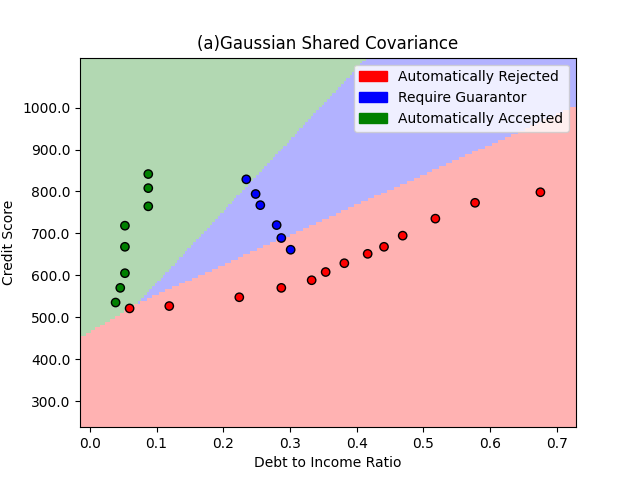
\includegraphics[width=0.5\linewidth]{hw2/(a)Gaussian Shared Covariance.png}
\end{figure}
\begin{figure}[H]
    \centering
    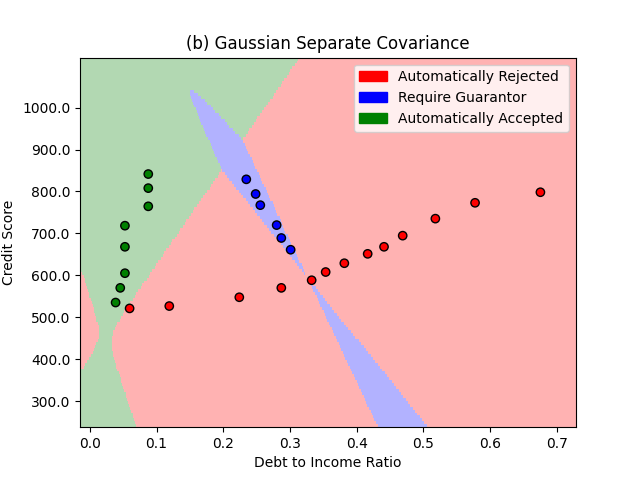
\includegraphics[width=0.5\linewidth]{hw2/(b) Gaussian Separate Covariance.png}
\end{figure}
\begin{figure}[H]
    \centering
    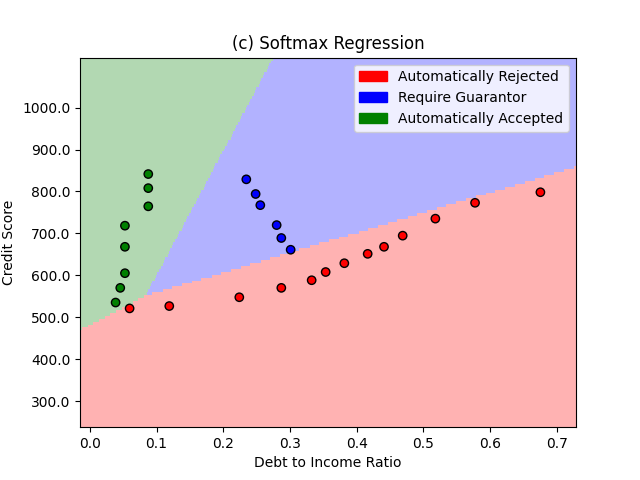
\includegraphics[width=0.5\linewidth]{hw2/(c) Softmax Regression.png}
\end{figure}
\begin{figure}[H]
    \centering
    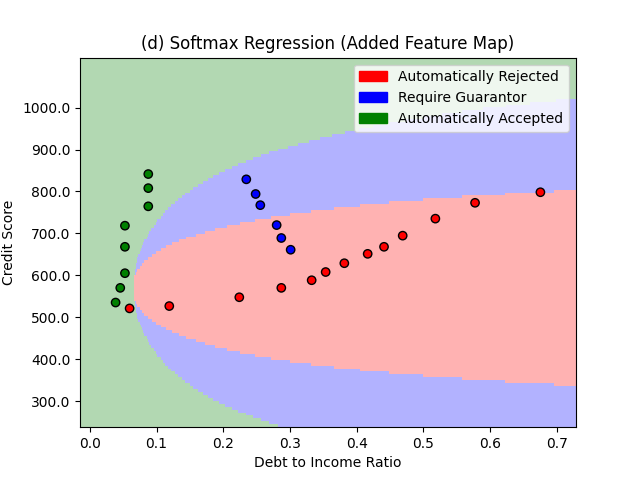
\includegraphics[width=0.5\linewidth]{hw2/(d) Softmax Regression (Added Feature Map).png}
\end{figure}
\begin{figure}[H]
    \centering
    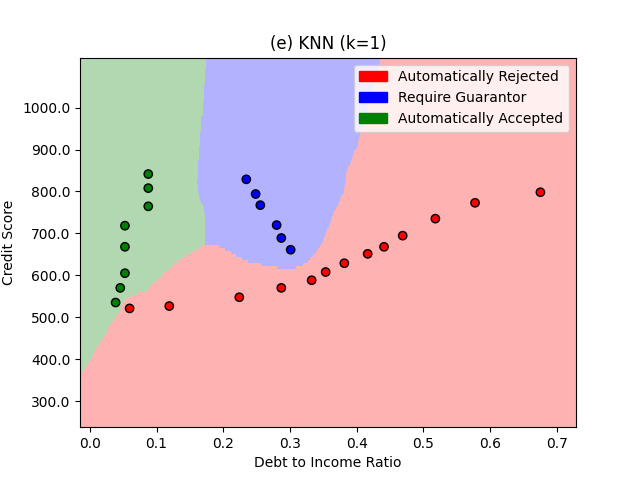
\includegraphics[width=0.5\linewidth]{hw2/(e) KNN (k=1).png}
\end{figure}
\begin{figure}[H]
    \centering
    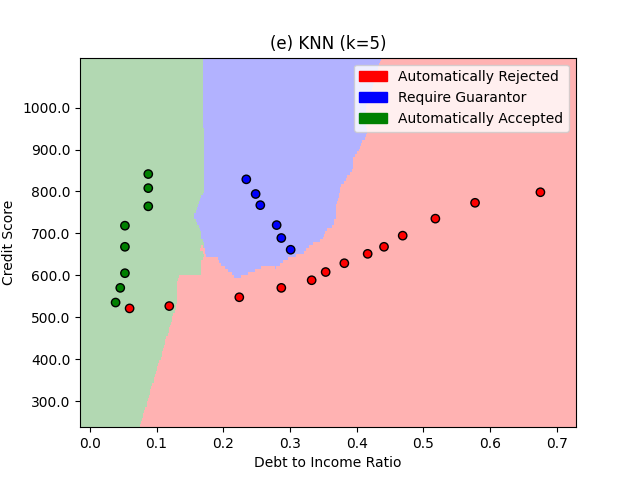
\includegraphics[width=0.5\linewidth]{hw2/(e) KNN (k=5).png}
\end{figure}

The models perform their classifications differently. The Guassian generative model with shared covariance matrices seem to have linear boundaries between the classifications, which seems to arise because of the shared covariances. Meanwhile, Guassian generative models with separate covariances seem to have almost elliptical/parabolic class boundaries due to the separate covariances, which allow it to more accurately capture the data. The default softmax regression is a linear classifier that has a decision boundary on a hyperplane. However, adding the feature map (the log and square transformations above) result in nonlinear and decision boundaries which in this case do not seem to perform better since a linear boundary is sufficient for the training data. Finally, the kNN classifier for $k=1$ has rigid boundaries since it is solely based on the first nearest neighbor to any datapoint. Surprisingly, the kNN for $k=5$ seems to have a more jagged decision boundary which overlaps classes with datapoints since it works based on a "voting" system where the most common neighbor among the 5 closest will be the class decision. This leads to some apparent misses but actually testing this would require more data.


\item For a new loan applicant we can see the classifications for the two models.

\begin{itemize}
    \item (c): class 0 with probability of 1. In other words, \textbf{Automatically Rejected} with probability \textbf{1}.

    \item (d): class 1 with probability 0.78023571. In other words, \textbf{Require Guarantor} with probability \textbf{0.7802}. class 0 with probability of 0.219692184. In other words, \textbf{Automatically Rejected} with probability \textbf{0.2197}.
\end{itemize}

Our model (c) flatout rejects the applicant since the credit score and debt ratio in the training data result in a near 100\% correlation for rejection. This can be viewed above int he softmax regression plot where this point would be comfortably in the red region. However, our model (d) has a high chance of requiring a guarantor, although it is not as certain as the first model since it accounts for nonlinear features mapping. This can be observed above in the plots where the datapoint would be in the blue region but also be close to the other two as well, which could lead to some uncertainty. As modelers, we should be aware that making predictions on far away points by extrapolating from the training data could be misleading since there is little data in those regions to truly determine which features should lead to what outcomes.

\item Using a classifier trained on past decisions may miss important external context such as unexpected financial difficulties or future potential cash flow. This would result in people who could truly use a loan and would be able to pay it back being automatically rejected in some cases. Additionally, depending on the training data that we use, we could introduce bias if it existed in the training. This would only perpetuate existing problems. There could be cases where someone has low credit score but now a high income due to education etc. in which they would be able to pay off the loan but because of their previous credit score, are unable to get one (for example, someone who just finished medical school will have to go through residency but in the future has high growth potential). Judging solely on past decisions could help inform decisions but using it as a sole determinant without any human oversight or input could result in unfair outcomes. Other variables such as employment history or previous medical bills could provide a better informed background in that can help in the decision making.



\end{enumerate}

\end{solution}

\newpage
%%%%%%%%%%%%%%%%%%%%%%%%%%%%%%%%%%%%%%%%%%%%%
% Name and Calibration
%%%%%%%%%%%%%%%%%%%%%%%%%%%%%%%%%%%%%%%%%%%%%
\newpage

\textbf{Name}: Charles Zhou

\textbf{Collaborators and Resources}: 

\end{document}
